\chapter{Introduction}
\label{chap:intro}

\section{Charge Transport in Organic Semiconductors}
\subsection{Organic Semiconductors}
Conductive polymers were first discovered in 1977 by Shirakawa et al  \cite{chiang_electrical_1977, Shirakawa1977Jan} for which they were awarded the Nobel prize in Chemistry. Recently these materials have become ubiquitous in many technologies, such as in organic photovoltaic cells\cite{Kippelen2009}, organic field-effect transistors (OFET) \cite{Malachowski2010Jun} and organic light-emitting diodes (OLED) \cite{ThejoKalyani2012Jun}. While the other two technologies lag behind their inorganic counterparts, uptake of OLED screens is becoming ubiquitous -especially in the smartphone and television market due to their flexibility, better colour representation and lower energy consumption than standard backlit LCD displays. OLEDs have also found uses in lighting with their efficiency rivalling that of fluorescent tubes \cite{Reineke2009May, OLED_lighting}. Although, industry has made large strides in fabricating and using these materials the exact nature of the charge transport is still poorly understood. Traditional theories (such as hopping and band transport) aren't applicable to many relevant materials \cite{coropceanu_charge_2007, Giannini2019, C0CS00198H, Fratini_2016, yavuz_dichotomy_2017} as charge transfer dynamics lies in an intermediate region where the polaron is neither fully localised or delocalised. This is due to crystals typically being formed of organic molecules weakly held together by Van der Waals (VDW) forces rather than strong covalent bonds. This allows molecules to fluctuate about their lattice sites and introduces a disorder that doesn't appear in inorganic crystals. 
\\\\
In order to properly quantify the performance of organic semiconductors a key property is the charge carrier mobility. Typically, charge carrier mobilities in `good' organic semiconductors (OSCs) fall between 1-10 cm$^2$V$^{-1}$s$^{-1}$ \cite{Brown2018Mar}. Though higher mobilities, in pure crystals such as Rubrene, have been recorded in the range 15-20+ cm$^2$V$^{-1}$s$^{-1}$ \cite{Zimmerling_RubMob, Podzorov_Rubrene}. This is beyond the range of hopping model validity ($\sim$1 cm$^2$V$^{-1}$s$^{-1}$) and below that of band theory ($>$ 50 cm$^2$V$^{-1}$s$^{-1}$) \cite{yavuz_dichotomy_2017}. In this intermediate regime the charge carriers are typically not completely delocalised at the valence band edges (band regime) or localised to a single site/molecule (hopping regime) but delocalised over a few/tens of molecules \cite{giannini_crossover_2018}. Without any analytic approaches currently being valid in this regime many atomistic computational approaches have been developed to investigate the underlying charge transport mechanisms\cite{oberhofer_charge_2017}.
\\\\
\section{Atomistic Simulations of Nonadiabatic Processes}
In simulating processes involving electronic transfers a key approximation used in conventional molecular dynamics (MD) breaks down. That is the Born-Oppenheimer or adiabatic approximation \cite{john_c._tully_nonadiabatic_nodate}. This approximation, relied upon for almost a century \cite{Pisana2007Feb}, hinges on the fact that nuclei are much more massive than electrons and are approximately stationary with respect to electron movement \cite{Born1927Jan}. This results in nuclear evolution that is governed by a single, adiabatic, potential energy surface. However, in many interesting processes, such as the proton coupled electron transfer in photosynthesis and respiration
 \cite{Hammes-Schiffer2001Apr, Hammes-Schiffer1994Sep, Huynh2007}, non-radiative decay and photochemical processes, electronic transitions between adiabatic potential energy surfaces occur \cite{tully_nonadiabatic_1991}. Simulating these processes requires non-adiabatic molecular dynamics (NAMD) techniques to be developed, to correctly capture dynamical properties.
\\\\
There have been many techniques proposed for use in NAMD such as the quantum classical Louiville equation \cite{Kapral1999May}, multiple spawning \cite{Martnnez*2005Oct} or nonadiabatic Bohmian dynamics \cite{Albareda2014Aug}. However, two of the most popular are trajectory surface hopping \cite{Tully1990Jul} and mean-field approaches \cite{Whetten85}. This is probably due to their relative simplicity to implement, efficiency for large systems and proven efficacy in a wide variety of situations
\cite{Shenvi2011Apr}. In these approaches the general aim is to treat as much of the system as possible with (computationally cheaper) classical mechanics. While handling all necessary parts with quantum mechanics \cite{Coker1995Jan}. In Surface Hopping, Ehrenfest and Coupled-Trajectory Mixed Quantum-Classical molecular dynamics (CTMQC) one treats the nuclear subsystem classically and the electronic one quantum mechanically. The nuclei are normally propagated using a velocity verlet algorithm according to Newton's laws and electrons using a fourth order Runge Kutta algorithm according to the time-dependent Schr\"odinger equation. The wavefunction is normally expanded as a linear combination of adiabatic or diabatic states. The nuclei and electrons can also interact. Taking account of this interaction is where these techniques differ. No one technique is perfect, the issues for surface hopping and Ehrenfest are well documented and have been discussed in detail \cite{SubotnikReview2016, Giovanni_2010_deco, Jaeger_2012_deco, Jain2016, Subotnik_2011_deco}. CTMQC is a fairly new technique and its issues are still mostly unknown. In this document I will discuss CTMQC in depth and present results from my own implementation of it as well as presenting its drawbacks. I will also compare these results to Ehrenfest and Trajectory Surface Hopping (TSH).
\subsection{Surface Hopping and Ehrenfest Dynamics \label{sec:Ehren_SH}}
\begin{wrapfigure}{r}{0.45\textwidth}
  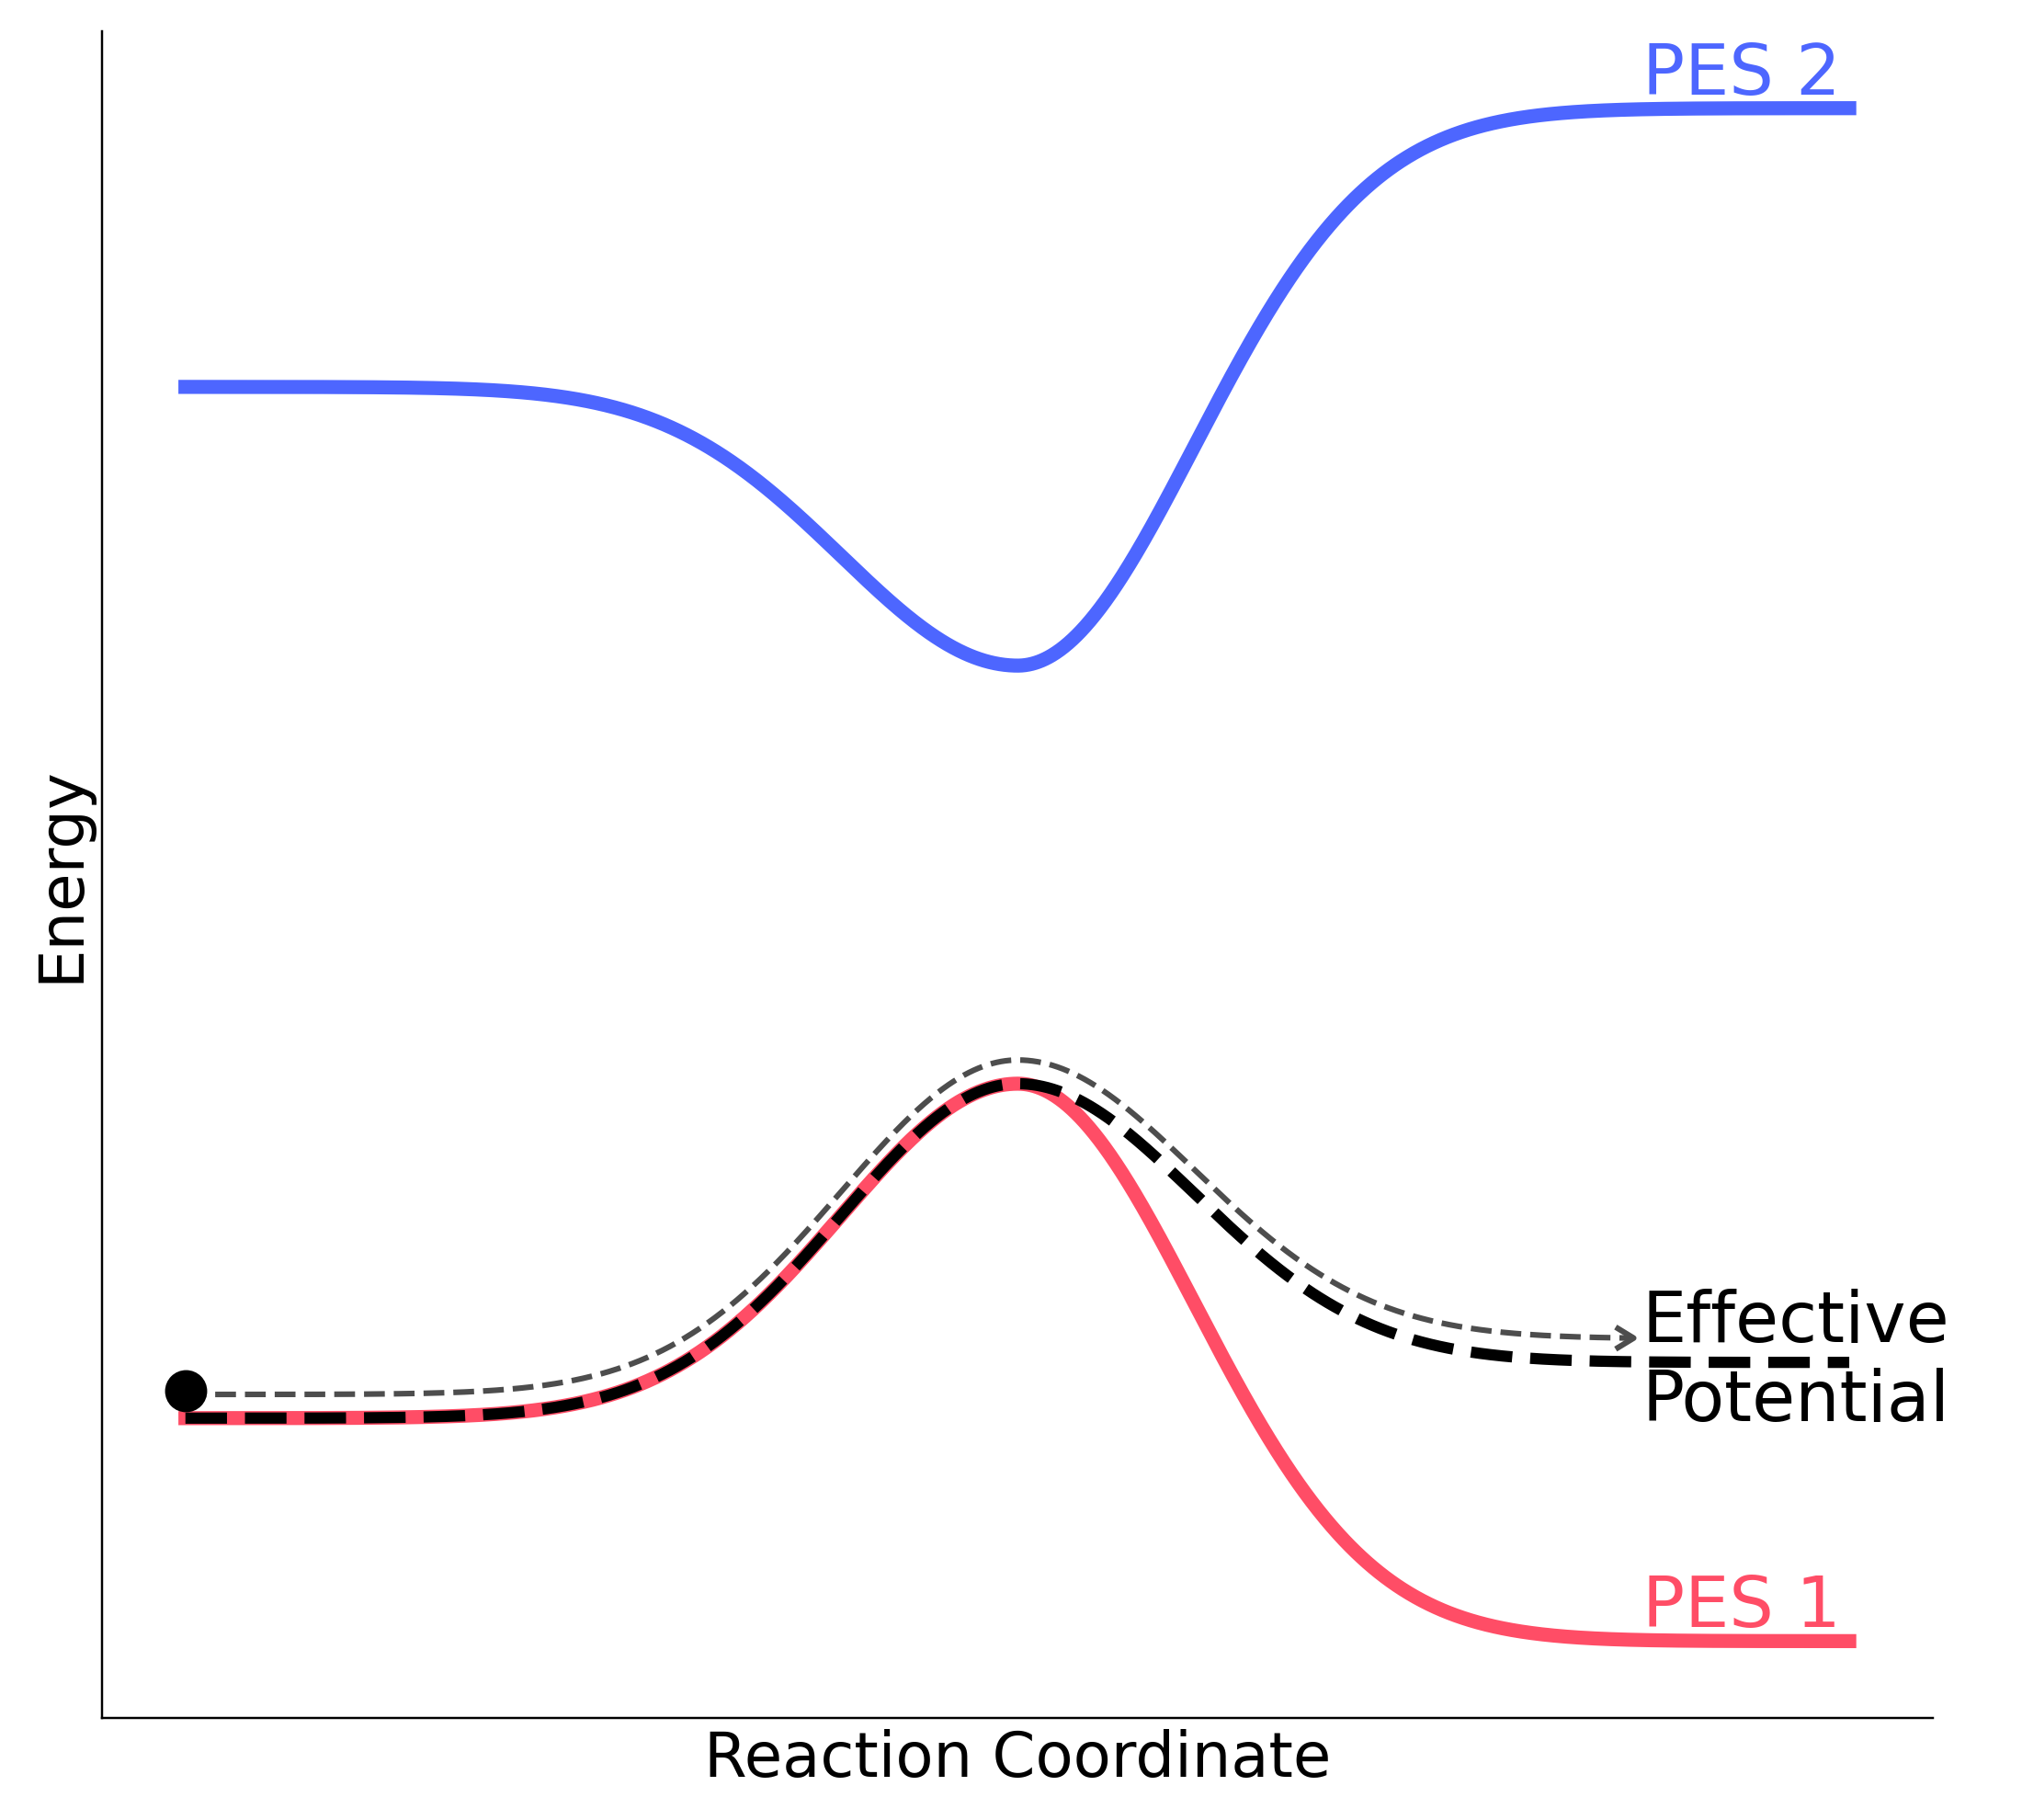
\includegraphics[width=0.45\textwidth]{./img/Eh_hop.png}
  \caption{\label{fig:Eh_diag}An example of a typical Ehrenfest simulation near an avoided crossing. The black lines represent the adiabatic potential energy surface due to the ground (PES 1) and excited (PES 2) state. The red line represents the population weighted average potential the nuclei travel on.}
\end{wrapfigure}
An important technique in the field of mixed quantum classical nonadiabatic molecular dynamics is Ehrenfest dynamics. Assuming we treat the nuclei classically the Ehrenfest equations can be rigorously derived from the electronic Schr\"odinger equation. This is done by assuming that the nuclei's motion is provided by a single population weighted average potential energy surface. This average is taken from the adiabatic potential energy surfaces (eigenvalues of the Hamiltonian) where weights are provided by the populations of each adiabatic state. This effective potential energy surface is shown in fig \ref{fig:Eh_diag}. In this way the electronic subsystem influences the propagation of the nuclei. The propagation of the forces and the electrons are controlled by equations \eqref{eq:Eh_Force} and \eqref{eq:Eh_Elec}.
\\
\begin{equation}
  F_{\nu}^{Ehren} = \sum_i^{N_{st}} |C_{i}|^2 \nabla_{\nu} E_{i} + \sum_{i,j}^{N_{st}} C_{i}^{*} C_{j} (E_{j} - E_{i}) \textbf{d}_{ij, \nu}
  \label{eq:Eh_Force}
\end{equation}
\begin{equation}
  i \hbar \vec{C}_{m} = C_{m}E_{m} -  i \ \hbar  \sum_{n}^{N_{st}} C_{n} d^{ad}_{mn}
  \label{eq:Eh_Elec}
\end{equation}
In the above equations $C_{i}$ is the adiabatic expansion coefficient for state i, $E_{m}$ is the energy of adiabatic state m, $\textbf{d}_{mn, \nu}^{ad}$ is the nonadiabatic coupling (in the adiabatic basis) between states m and n for atom $\nu$. The $d_{mn}^{ad}$ are the nonadiabatic coupling elements expressed in the adiabatic basis.
Although the Ehrenfest method has been applied with success in many systems \cite{Li2005Aug, Saita2012Dec, Kohen1998Sep} it has a number of key shortcomings. Namely, its inability to capture the branching of the nuclear wavefunction as propagation occurs on only a single potential energy surface and its poor account of the decoherence of the electronic and nuclear subsystem after an avoided crossing. Ehrenfest also violates detailed balance by populating all adiabatic states evenly \cite{tully_perspective:_2012, john_c._tully_nonadiabatic_nodate}. In the limit of infinite states this results in infinite electronic temperature \cite{parandekar_detailed_2006}.
\begin{wrapfigure}{r}{0.45\textwidth}
  \includegraphics[width=0.45\textwidth]{./img/SH_hop.png}
  \caption{\label{fig:SH_diag}An example of a typical Surface Hopping simulation near an avoided crossing. The black lines represent the adiabatic potential energy surface due to the ground (PES 1) and excited (PES 2) state. The red line represents the discontinuous effective potential the nuclei travel on.}
\end{wrapfigure}
\noindent Possibly the most popular technique in NAMD is trajectory surface hopping. In trajectory surface hopping the shape of the potential energy surface is determined by a series of discrete stochastic hops between adiabatic potential energy surfaces \cite{tully_perspective:_2012}. See fig \ref{fig:SH_diag}.  The probability of these hops is determined by the non-adiabatic coupling between states.
A swarm of trajectories are used and the probability a hop (non-adiabatic coupling) determines how many of these change state. The nuclear dynamics are dictated by the shape of the energy surface they are travelling on. This method can capture the branching of nuclear wavepacket unlike Ehrenfest. However, it still suffers from a number of issues. The original `fewest switches surface hopping' proposed by John Tully suffered from bad overcoherence of the nuclear and electronic subsystems. That is the electronic and nuclear motion was coupled long after the region of high non-adiabatic coupling (crossing region). The fact that the hops are instant leads to discontinuities and methods need to be implemented to fix these such as velocity re-scaling. Finally, perhaps the most important shortcoming is that this technique has not been derived from first principles and cannot be guaranteed to work generally. These problems have lead to a number of other techniques being developed. One of these, CTMQC, is the subject of this report.

